In this section, we describe how the domain decomposition and the
exchange of particles are implemented in FDPS.  We use the
three-dimensional multi-section
decomposition \cite{2004PASJ...56..521M} as the method for the domain
decomposition in FDPS.  In this method, first we construct a cuboid
which covers all particles. We call this cuboid the computational
domain. When the periodic boundary condition is used, the dimensions
of this cuboid is given from the user program. In the case of an open
boundary, FDPS constructs the dimensions from positions of
particles. This computational domain is then divided into $n_x$
domains by planes perpendicular to the $x$-axis. Each of these $n_x$
domains is then further subdivided into $n_y$ domains by planes
perpendicular to the $y$-axis, and finally the same thing is done for
the $z$-axis.  In each step, the division is made so that the
computational load is equally distributed to all subdomains. We will
discuss this point in more details below.

Figure~\ref{fig:decomposition} illustrates the result of the
multi-section decomposition with $(n_x, n_y, n_z)=(7,6,1)$. We can see
that the size and shape of subdomains shows large variation. By
allowing this variation, FDPS achieves quite good load balance and
high scalability.  Note that $n=n_x n_y n_z$ is the number of MPI
processes. By default, values of $n_x$, $n_y$, and $n_z$ are chosen so
that they are integers close to $n^{1/3}$. For figure
~\ref{fig:decomposition}, we force the numbers used to make
two-dimensional decomposition.

\begin{figure}
  \begin{center}
    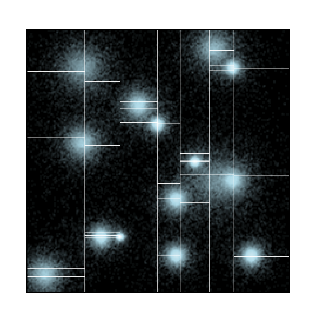
\includegraphics[width=8cm]{fig/pm3d.eps}
  \end{center}
  \caption{Example of the domain decomposition. The division is $7
    \times 6$ in 2-dimension.}
  \label{fig:decomposition}
\end{figure}

In the following, we describe how the calculation of the geometry of
subdomains (we denote this part as ``domain decomposition'') and the
exchange of particles are implemented in FDPS.  They correspond to the
member function \texttt{decomposeDomainAll} of class \texttt{DomainInfo} and
\texttt{exchangeParticle} of class \texttt{ParticleSystem}.

We adopts the ``sampling
method'' \cite{Blackston:1997:HPE:509593.509597} for the domain
decomposition, which consists of the following steps:
\begin{enumerate} 
\item Each process samples particles randomly from its own
  particles. In order to achieve the optimal load balance, the
  sampling rate of particles is changed so that it is proportional to
  the CPU time per particle spent on that
  process \cite{ishiyama:greem}. FDPS provides several options
  including this optimal balance. \label{proc:sampling}
%%
\item Each process sends their sample particles to the process with
  rank 0. Hereafter, we call this process ``root
  process''. \label{proc:gathering}
%%
\item The root process determines the new candidate subdomains  by
applying  the following procedure to x, y, and z coordinates.
 \label{proc:sorting}
%%
  \begin{itemize}
%%
  \item Sorts the sampled particles in the domain (or subdomains
    created in the previous steps) using 
    their coordinates used in the current step, 
    and divide particles into 
    $n_k$ subsets ($k$ is the coordinate axis for the current step).
    with equal number of sample particles.
  \end{itemize}
%%
\item The root process determines the final subdomains by applying the
    weighted average between the previous one and the new candidate. This
    procedure is used to stabilize the decomposition and suppress
    unnecessary oscillation. \label{proc:moving}
%%
\item The root process broadcasts the geometries of the final
    subdomains  to
  all the other processes. \label{proc:broadcasting}
%%
\end{enumerate}

The advantage of the sampling method is in its low calculation and
communication cost. They are $\mathcal{O}(N_\mathrm{s} \log
N_\mathrm{s})$ and $\mathcal{O}(N_\mathrm{s} )$, where $N_\mathrm{s}$
is the total number of sampled particles. Thus, as far as
$N_\mathrm{s}$ is not much larger than $N/n$, the average number of
particles per process, the cost of domain decomposition is negligible.

After the domain decomposition is done and the result is broadcasted
to all processes, they exchange particles so that each of them has the
particles in its domain. Since each process has the complete
information of the domain decomposition, this part is pretty
straightforward to implement. Each process looks at each of its
particles, and determines if that particle is still in its domain.  If
not, the process determines to which process that particle should be
sent. After the destinations of all particles are determined, each
process sends them out, using \texttt{MPI\_Alltoallv} function.

% LocalWords:  FDPS subdomain MPI multi subdomains DomainInfo ParticleSystem
% LocalWords:  decomposeDomainAll exchangeParticle substeps scalability
% LocalWords:  broadcasted Alltoallv
